\documentclass["../Cours.tex"]{subfiles}

\begin{document}
\chapitre{Solides de l'espace, volumes et contenance}

\definition{Un solide est un objet de l'espace, possédant trois dimensions : longueur, largeur, hauteur.\\La face d'un solide est une figure plane, en deux dimensions, qui le délimite.\\Une arête est un segment commun à deux faces.\\Un sommet est le point commun à plusieurs arêtes.}

\begin{center}
    \begin{tikzpicture}
        \draw[fill=gris] (3,0) -- ((3,3) -- (4,4) -- (4,1) -- cycle;
        \draw (0,3) -- (3,3) -- (3,0) -- (0,0);
        \draw (1,4) -- (4,4)  (4,1) -- (4,4);
        \draw (0,3) -- (1,4) (3,3) -- (4,4) (3,0) -- (4,1);
        \draw[dashed] (0,0) -- (1,1) (4,1) -- (1,1) -- (1,4);
        
        \draw[latex-] (3.5,2) -- (5,2);
        \node[anchor=west] at (5,2) {face};
        \draw[latex-] (4,4) -- (5,4);
        \node[anchor=west] at (5,4) {sommet};
        \draw[thick, rouge] (0,0) -- (0,3);
        \draw[-latex] (-2,2) -- (0,2);
        \node[anchor=east] at (-2,2) {arête};
    \end{tikzpicture}
\end{center}

\partie{Volume et contenance}

\definition{Le volume d'un solide mesure l'intérieur d'un solide, une partie de l'espace.}

\convention{Dans le Système International (SI) d'unités, l'unité du volume est le \unit{\metre\cube}.}


\partie{Solides de l'espace}
\souspartie{Polyèdres}

\definition{Un polyèdre est un solide dont toutes les faces sont des polygones}

\soussouspartie{Le cube}

\definition{Un cube (aussi appelé hexaèdre régulier) est un polyèdre à 6 faces, 8 sommets et 12 arêtes. Toutes les faces sont des carrés.}

\formule{Si le cube est d'arête $c$ : $$V_{cube} = c \times c \times c$$}

\begin{figure}[h!]
    \centering
    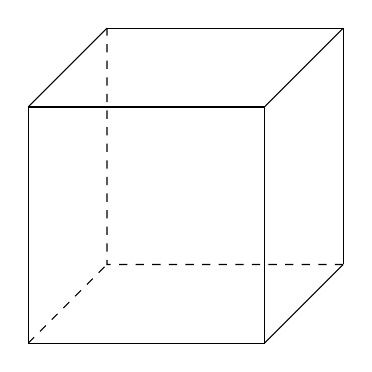
\begin{tikzpicture}
        \draw (0,3) -- (3,3) -- (3,0) -- (0,0) -- cycle;
        \draw (1,4) -- (4,4)  (4,1) -- (4,4);
        \draw (0,3) -- (1,4) (3,3) -- (4,4) (3,0) -- (4,1);
        \draw[dashed] (0,0) -- (1,1) (4,1) -- (1,1) -- (1,4);
    \end{tikzpicture}
    \caption{Représentation en perspective cavalière d'un cube}
    \label{fig:chapitre4_cube}
\end{figure}

\soussouspartie{Le pavé droit}

\definition{Un pavé droit (ou parallélépipède rectangle) est un hexaèdre (un polyèdre à 6 facess) dont toutes les faces sont des rectangles. Il possède 8 sommets et 12 arêtes.}

\formule{Si le pavé droit est le longueur $L$, de largeur $l$ et de hauteur $h$ : }

\begin{figure}[h!]
    \centering
    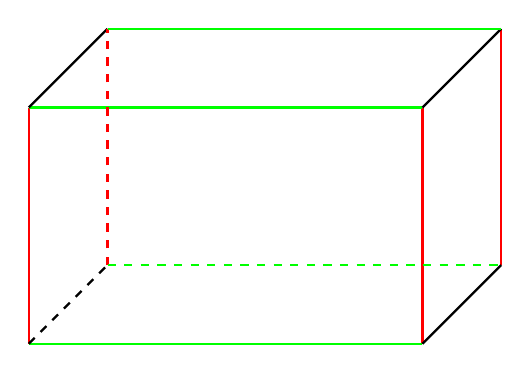
\begin{tikzpicture}
        \draw[thick,red] (0,0) -- (0,3) (5,0) -- (5,3) (6,1) -- (6,4);
        \draw[thick,green] (0,0) -- (5,0) (0,3) -- (5,3);
        \draw[thick,] (5,0) -- (6,1) (5,3) -- (6,4) (0,3) -- (1,4);
        \draw[thick,dashed] (0,0) -- (1,1);
        \draw[thick,dashed,red] (1,1) -- (1,4);
        \draw[thick,dashed,green] (1,1) -- (6,1);
        \draw[thick,green] (1,4) -- (6,4);
    \end{tikzpicture}
    \caption{Représentation en perspective cavalière d'un pavé droit}
    \label{fig:chapitre4_pavedroit}
\end{figure}

\soussouspartie{La pyramide}

\definition{Une pyramide est un polyèdre dont une face appelée la base est un polygone, et dont tous les sommets de la base sont reliés en un point appelé l'apex.}

\begin{figure}[h!]
    \centering
    \begin{tikzpicture}
        \coordinate (A) at (0,0);
        \coordinate (B) at (4,0);
        \coordinate (C) at (2,-2);
        \coordinate (D) at (2.5,4);
        \shadedraw[top color=gris, bottom color=grisclair] (A) -- (B) -- (C) -- cycle;
        \draw[thick] (D) -- (A) -- (C) -- (B) -- (D) -- (C);
        \draw[dashed,thick] (A) -- (B);
        \draw[latex-] ($(D)+(0.2,0)$) -- ($(D)+(2,0)$);
        \node[anchor=west] at ($(D)+(2,0)$) {apex};
        \draw[latex-] ($(C)+(0.5,1)$) -- ($(C)+(2.5,1)$);
        \node[anchor=west] at ($(C)+(2.5,1)$) {base};
    \end{tikzpicture}
    \caption{Représentation en perspective cavalière d'une pyramide à base triangulaire}
    \label{fig:chapitre4_pyramidebasetriangulaire}
\end{figure}

\soussouspartie{Le prisme droit}

\definition{Un prisme droit est un polyèdre dont deux des faces - les bases - sont superposables (de même dimensions) et parallèles, et dont toutes les faces latérales sont des rectangles.}

\begin{figure}[h!]
    \centering
    \begin{tikzpicture}[scale=3]
        \coordinate (A) at (0,0);
        \coordinate (B) at (0.2,0.3);
        \coordinate (C) at (0.6,0.3); 
        \coordinate (D) at (1,0.2);
        \coordinate (E) at (0.7,0);
        \coordinate (A') at (0,1);
        \coordinate (B') at (0.2,1.3);
        \coordinate (C') at (0.6,1.3); 
        \coordinate (D') at (1,1.2);
        \coordinate (E') at (0.7,1);
        \draw[white,fill=gris] (A) -- (B) -- (C) -- (D) -- (E) -- cycle;
        \draw[white,fill=gris] (A') -- (B') -- (C') -- (D') -- (E') -- cycle;
        
        \draw[dashed] (A) -- (B) -- (C) -- (D);
        \draw (D) -- (E) -- (A);
        \draw (A') -- (B') -- (C') -- (D') -- (E') -- cycle;
        \draw (A) -- (A') (D) -- (D') (E) -- (E');
        \draw[dashed] (B) -- (B') (C) -- (C');
        
        \draw[latex-] (0.5,1.1) -- (1.5,1.1) node[anchor=west] {base};
        \draw[latex-] (0.5,0.1) -- (1.5,0.1) node[anchor=west] {base};
        \draw[latex-latex] (-0.1,0) -- (-0.1,1);
        \draw (-0.1,0.5) node[anchor=east] {hauteur};
        
    \end{tikzpicture}
    \caption{Représentation en perspective cavalière d'un prisme droit à base pentagonale}
    \label{fig:my_label}
\end{figure}

\formule{$$\curs{V}_{\mbox{prisme droit}} = \curs{A}_{\mbox{base}} \times \mbox{hauteur}$$}


\souspartie{Solides de révolution}

\definition{Un solide de révolution est engendré par une surface plane tournant autour d'un axe.}

\soussouspartie{Le cylindre de révolution}

\definition{Un cylindre est un solide de révolution obtenu en faisant tourner un rectangle autour d'un de ses côtés.}

\begin{figure}[h!]
    \centering
    \begin{tikzpicture}[scale=0.7]
        \coordinate (A) at (0,0);
        \coordinate (B) at ($(A)+(1.5,0)$);
        \coordinate (C) at ($(A)+(1.5,3)$);
        \coordinate (D) at ($(A)+(0,3)$);
        \draw (A) -- (B) -- (C) -- (D) -- cycle;
        \draw[thick,red] ($(B)+(0,-0.8)$) -- ($(C)+(0,0.5)$);

        \coordinate (A) at (3,0);
        \coordinate (B) at ($(A)+(1.5,0)$);
        \coordinate (C) at ($(A)+(1.5,3)$);
        \coordinate (D) at ($(A)+(0,3)$);   
        \draw (A) -- (B) -- (C) -- (D) -- cycle;
        \draw[thick,red] ($(B)+(0,-0.8)$) -- ($(C)+(0,0.5)$);
        \draw (B) ellipse (1.5 and 0.5);
        
        \coordinate (E) at ($(A)+(0.3,-0.3)$);
        \coordinate (F) at ($(E)+(0,3)$);
        \draw (C) -- (F) -- (E) -- (B);
        
        \coordinate (A) at (7,0);
        \coordinate (B) at ($(A)+(1.5,0)$);
        \coordinate (C) at ($(A)+(1.5,3)$);
        \coordinate (D) at ($(A)+(0,3)$);   
        \draw (A) -- (B) -- (C) -- (D) -- cycle;
        \draw[thick,red] ($(B)+(0,-0.8)$) -- ($(C)+(0,0.5)$);
        \draw (B) ellipse (1.5 and 0.5);
        \draw (C) ellipse (1.5 and 0.5);
        \draw (B) -- ($(A)+(3,0)$) -- ($(D)+(3,0)$) -- (C);
        
        \coordinate (E) at ($(A)+(0.3,-0.3)$);
        \coordinate (F) at ($(E)+(0,3)$);
        \draw (C) -- (F) -- (E) -- (B);
        \coordinate (E) at ($(A)+(0.3,0.3)$);
        \coordinate (F) at ($(E)+(0,3)$);
        \draw (C) -- (F) -- (E) -- (B);
        \coordinate (E) at ($(A)+(2.7,0.3)$);
        \coordinate (F) at ($(E)+(0,3)$);
        \draw (C) -- (F) -- (E) -- (B);
        \coordinate (E) at ($(A)+(2.7,-0.3)$);
        \coordinate (F) at ($(E)+(0,3)$);
        \draw (C) -- (F) -- (E) -- (B);
        \coordinate (E) at ($(A)+(1.3,-0.5)$);
        \coordinate (F) at ($(E)+(0,3)$);
        \draw (C) -- (F) -- (E) -- (B);
        \coordinate (E) at ($(A)+(1.7,-0.5)$);
        \coordinate (F) at ($(E)+(0,3)$);
        \draw (C) -- (F) -- (E) -- (B);
        
        \coordinate (A) at (12,0);
        \coordinate (B) at ($(A)+(1.5,0)$);
        \coordinate (C) at ($(A)+(1.5,3)$);
        \coordinate (D) at ($(A)+(0,3)$);
        \draw (A) -- (D) ($(A)+(3,0)$) -- ($(D)+(3,0)$);
        \draw (B) ellipse (1.5 and 0.5);
        \draw[white,fill=white] ($(A)+(0.03,0)$) rectangle ($(A)+(2.97,0.6)$);
        \draw (C) ellipse (1.5 and 0.5);
        \draw[dashed] (B) ellipse (1.5 and 0.5);
    \end{tikzpicture}
    \caption{Construction d'un cylindre par révolution autour d'un des côtés du rectangle}
    \label{fig:chapitre4_cylindre}
\end{figure}

\formule{$$V_{\mbox{cylindre}} = \pi \times \mbox{rayon}^2 \times \mbox{hauteur} $$}


\soussouspartie{Le cône de révolution}

\definition{Un cône est un solide de révolution obtenu en faisant tourner un triangle rectangle autour d'un des deux côtés qui ne sont pas l'hypoténuse.}

\begin{figure}[h!]
    \centering
    \begin{tikzpicture}[scale=0.6]
        % Figure 1
        \coordinate (O) at (0,0);
        \coordinate (A) at ($(O)+(-1.5,0)$);
        \coordinate (S) at ($(O)+(0,3)$);
        
        \draw[red,thick] ($(O)+(0,-1)$) -- ($(O)+(0,4)$);
        \draw (O) -- (A) -- (S) -- cycle;
        
        % Figure 2
        \coordinate (O) at (3,0);
        \coordinate (A) at ($(O)+(-1.5,0)$);
        \coordinate (S) at ($(O)+(0,3)$);
        
        \draw[red,thick] ($(O)+(0,-1)$) -- ($(O)+(0,4)$);
        \draw (O) -- (A) -- (S);
        \draw (O) ellipse (1.5 and 0.5);
        \draw (O) -- ($(O)+(-1.2,-0.3)$) -- (S);
        
        % Figure 3
        \coordinate (O) at (7,0);
        \coordinate (A) at ($(O)+(-1.5,0)$);
        \coordinate (S) at ($(O)+(0,3)$);
        
        \draw[red,thick] ($(O)+(0,-1)$) -- ($(O)+(0,4)$);
        \draw (O) -- (A) -- (S);
        \draw (O) ellipse (1.5 and 0.5);
        \draw (O) -- ($(O)+(-1.2,-0.3)$) -- (S);
        \draw (O) -- ($(O)+(1.2,-0.3)$) -- (S);
        \draw (O) -- ($(O)+(1.2,0.3)$) -- (S);
        \draw (O) -- ($(O)+(-1.2,0.3)$) -- (S);
        \draw (O) -- ($(O)+(1.5,0)$) -- (S);
        
        % Figure 4
        \coordinate (O) at (11,0);
        \coordinate (A) at ($(O)+(-1.5,0)$);
        \coordinate (B) at ($(O)+(1.5,0)$);
        \coordinate (S) at ($(O)+(0,3)$);
        
        \draw (A) -- (S) -- (B) ;
        \draw (O) ellipse (1.5 and 0.5);
        \draw[white,fill=white] ($(A)+(0.01,0)$) -- ($(S)+(0,-1)$) -- ($(B)+(-0.01,0)$) -- cycle;
        \draw[dashed] (O) ellipse (1.5 and 0.5);

    \end{tikzpicture}
    \caption{Construction d'un cône par révolution autour d'un des côtés du triangle rectangle}
    \label{fig:chapitre4_cone}
\end{figure}

\soussouspartie{Sphère et boule}

\definition{Une sphère est constituée de l'ensemble des points  à égale distance de son centre.\\ Une boule est constituée de l'ensemble des points situées à une distance inférieure ou égale}

\begin{figure}[h!]
    \centering
    \begin{tikzpicture}[scale=0.6]
        \coordinate (O) at (0,0);
        \draw (O) circle (2);
        \draw[dashed] ($(O)+(2,0)$) arc [ start angle = 0, end angle = 180, x radius = 2, y radius = 0.5];
        \draw ($(O)-(2,0)$) arc [ start angle = 180, end angle = 360, x radius = 2, y radius = 0.5];
        
        \coordinate (O) at (5,0);
        \shadedraw[ball color=lightgray] (O) circle (2);
        \draw[dashed] ($(O)+(2,0)$) arc [ start angle = 0, end angle = 180, x radius = 2, y radius = 0.5];
        \draw ($(O)-(2,0)$) arc [ start angle = 180, end angle = 360, x radius = 2, y radius = 0.5];
    \end{tikzpicture}
    \caption{Sphère et boule en perspective cavalière}
    \label{fig:chapitre4_sphere_boule}
\end{figure}



\end{document}